\documentclass[f,bachelor,binding,twoside,palatino]{WeSTthesis}
% Please read the README.md file for additional information on the parameters and overall usage of WeSTthesis

\usepackage[english,ngerman]{babel}         % English and new German spelling
\usepackage[utf8]{inputenc}                 % correct input encoding
\usepackage[T1]{fontenc}                    % correct output encoding
\usepackage{graphicx}                       % enhanced support for graphics
\usepackage{tabularx}                       % more flexible tabular
\usepackage{amsfonts}                       % math fonts
\usepackage{amssymb}                        % math symbols
\usepackage{amsmath}                        % overall enhancements to math environment
\usepackage[ngerman]{babel}
\usepackage[babel,german=quotes]{csquotes}
\usepackage{url}

\def \ajax {AJAX}

\def \pjax {PJAX}
\def \pjaxRequest {PJAX-request}
\def \pjaxRequests {PJAX-requests}

\def \pjaxr {PJAXR}
\def \pjaxrRequest {PJAXR-request}
\def \pjaxrRequests {PJAXR-requests}

\def \httpRequest {HTTP-request}
\def \httpRequests {HTTP-requests}

\author{Jonas Braun}

\title{Server-side implementations of the PJAXR framework for smart Ajax applications}

\degreecourse{Informatik}

\firstreviewer{Prof. Dr. Steffen Staab}
\firstreviewerinfo{Institute for Web Science and Technologies}

\secondreviewer{René Pickhardt}
\secondreviewerinfo{Institute for Web Science and Technologies}


\begin{document}

% optional: change document language from ngerman to english
% \selectlanguage{english}

\maketitle %prints the cover page  an empty page if two-sided print
\pagenumbering{roman}

\tableofcontents

\varclearpage

% list of figures
% \listoffigures
% \varclearpage

\pagenumbering{arabic}

% beginning of the actual text section
\section{Introduction}
  \subsection{Preamble}
  This bachelor thesis deals with the problem of asynchronicity on web-platforms and takes a close look at one attempt called \pjaxr{}.
  It explains where it is suitable to use, which requirements are necessary and evaluates a few in this thesis developed server-side implementations.
  All load time analysis which is described in this thesis is computed with the example network speed of 16.000 kbit/s and a delay between the client and the server of 10ms.
  

  \subsection{\httpRequests{}}
    The world wide web has one main protocol to let web-browsers and web-servers communicate, the Hypertext Transfer Protocol (HTTP), which is built on top of the Transmission Control Protocol (TCP).
    TCP and so \httpRequests{} always start with a handshake to establish a connection before data is transferred.
    After this handshake, the client sends the request data to the web-server.
    This recognizes and interprets the request and if the requested resource is available, sends the according data back, otherwise it sends an error.
    Typically it renders data out of a database into a HTML-Template or to JSON and sends it back as the response.
	Afterwards the browser receives, interprets and displays the response data, which is most of the time HTML, CSS, images or scripts.

    \subsubsection{Load time analysis\label{httpLoadTime}}
      To improve the retrieval of websites it is important to look on what the loading time is spent for.
      A typical request has an execution time of about 200ms, depending on how far the distance is between server and client.
      In the world of computers 200ms, is a long time.
      E.g. in Video Games rendering 60 frames per second are needed in real time applications, which means about 17ms to compute and render a whole frame.
      To understand why requests need that much time a further look is needed:\\\\
      The time a handshake costs is quite the same as the RTT, the Round Trip Time.
      This is the time to physically send data from one end to another and back again.
      As computers getting faster and network interpretation does not effort much time anymore the RTT in the handshake is about two times the delay of the connection.\\\\
      Transportation of data costs at least the same amount of the connection instantiation. 
      This means out of the 200ms a request in our environment lasts, about 40ms are network-based delays.
      In HTTP 0.9 and HTTP 1.0\footnote{\url{http://tools.ietf.org/html/rfc2068#section-19.7.1.1}} without an additional HTTP-Header \enquote{Connection: Keep-Alive} every connection had to instantiate a new TCP connection and so to handshake. 
      In HTTP 1.1\footnote{\url{http://www.w3.org/Protocols/rfc2616/rfc2616-sec8.html#sec8.1}} the connection stays alive which reduces the load time by the handshake-delay.\\\\
      The rest of the time is taken by the web-server to handle the request. 
      Web architectures can have a huge variation of tasks: 
      From only delivering static data to complex dynamic content compositing. 
      The latter ones often use databases or even more complex backend services. 
      A request to one of them can cost about 1ms, having more expensive requirements, like queries using JOINS, etc. can cost much more.
      Depending on how dynamic a platform is, it can have up to 400 queries, sometimes even more. 
      Two of the most used Web-frameworks, Drupal and Wordpress, for example need 150 and more queries.
      Having an average delay of 1ms per backend-request 150 requests take about 150ms.
      This means about 75 percentage of the request load time is used for retrieving data in the backend.
      We now have about 10 percentage of the load time seen on network traffic and 75 percentage on backend requests. 
      To make web platforms as fast as possible this means it is desirable to have a minimum of backend requests on the web-server and due to the network delay a minimum of different requests by the client at the same time.


    \subsection{Dynamic content and synchronicity}
      Dynamic content in websites is content which is changed within an already fully loaded web page, without loading another full page including all resources. 
      The Client-server model, which is described in \ref{clientServerModel}, does not support dynamic changes of the content. 
      To retrieve new information the client has to request another full web page, including all resources and data which is necessary, which makes this model \enquote{synchronous}.
      An \enquote{asynchronous} model is able to change content dynamically without having to load a whole page. \ajax{}, specified in \ref{ajax}, is the most used asynchronous technique for web platforms, \pjax{} and \pjaxr{}, introduced in \ref{pjax} and \ref{pjaxr}, are built on top of \ajax{}, so they are asynchronous as well.
      

      \subsection{The history object\label{theHistoryObject}}
      The window.history\footnote{\url{https://developer.mozilla.org/de/docs/Web/Guide/DOM/Manipulating_the_browser_history}} object is a Javascript object, which represents the current browser history.
      It is a list containing every site the client visited in the current session.
      Each item consists of state data, a title and an URL.
      It has the methods .back(), .forward() and .go() which are needed to navigate in the history, incl.  the back- and forward-buttons of the browser.
      Additionally the methods .pushState() and .replaceState() give developers the opportunity to add or replace an item of the history list.
      By default, when loading a new page, the browser automatically invokes .pushState() to append a new item, the new state, to the list.
      This behavior is not the default behavior on \ajax-requests, so the developer has to use the two latter functions to activate the back- and forward-buttons in an asynchronous environment. \pjax{} and \pjaxr{} already consist of an integration like that.


  \subsection{Client-server model\label{clientServerModel}}
    The world wide web has one standard pattern which controls the data flow, the \enquote{Client-server model}.
    It defines that a client requests a web source via a \httpRequest{} including a URL and HTTP-headers which define what exactly the client wants to receive from the server.
    Afterwards all further resources, e.g. css, images, scripts, which are linked on this web source are requested.
    Any further request behaves in the exact same way, a full load of a page is always needed.

    \subsubsection{Load time analysis}
      The Client-server model has one initial \httpRequest{} to get the HTML-page and afterwards it has another request per resource linked in it. 
      As seen in \ref{httpLoadTime} a \httpRequest{} of a Wordpress page lasts about 200ms.
      Resources like CSS and scripts have typically small file-sizes.
      On modern pages an average file-size of all those resources are 100kb per page. 
      Because of the connection delay it is better to have a minimum of those resources, so they are typically combined together to one file per type.
      This means a typical CSS and script load time duration is about 25ms, the duration of a 100kB file transferred through 16k connection, plus another 40ms network delay.
      Overall a fully loaded web page including all resources takes 200ms + 130ms to be downloaded completely except for images which are typically loaded afterwards.\\
      In this classic model, changing the page causes another request of the same type, so it lasts the same time.
    
    \subsubsection{Requirements}
    This model does not have extra requirements.
    Only a HTTP-Server which can take \httpRequests{} is needed.

    \subsubsection{Example}
    TODO
      
    \subsubsection{Pro / Contra}
      \begin{itemize}
  	    \item[+]{The browser functionality is supported completely, especially the back- and forward-buttons.}
  	    \item[+]{This is the least complicated way to receive websites.}
        \item[-]{It is not possible to have dynamic content on the page.}
      \end{itemize}

    
  \subsection[\ajax]{\ajax{}\footnote{\url{https://developer.mozilla.org/de/docs/AJAX}}\label{ajax}}
    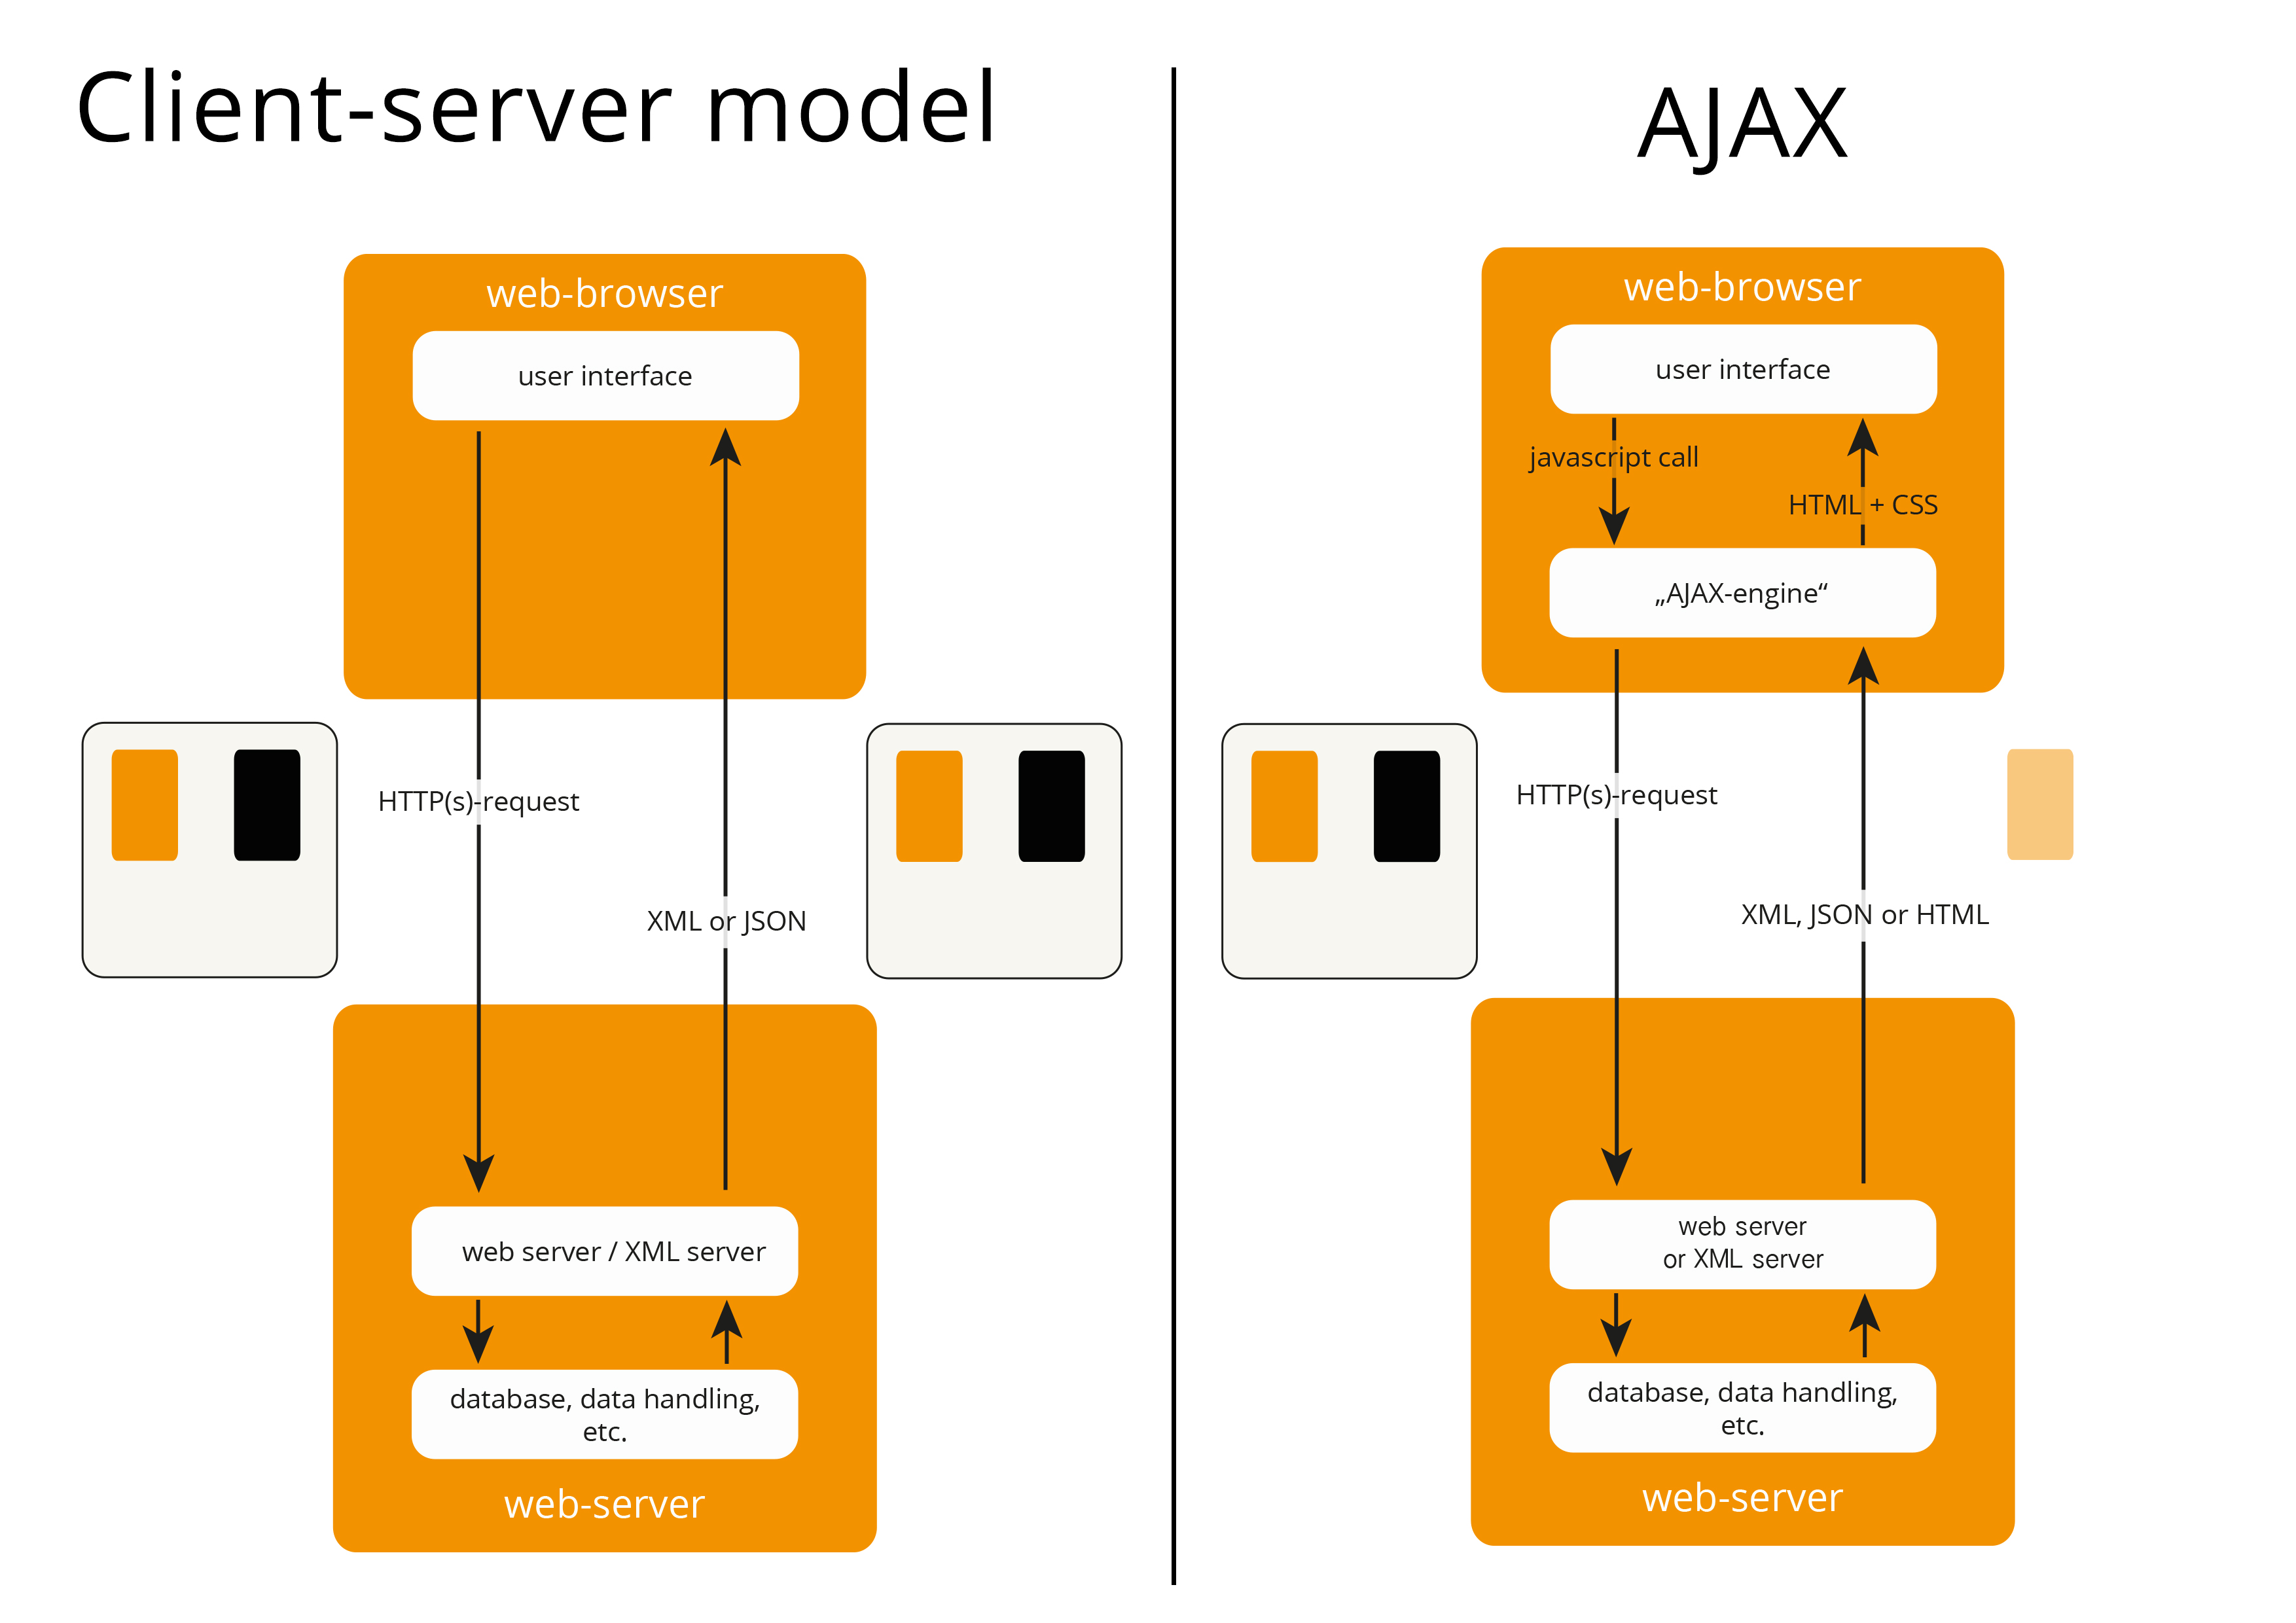
\includegraphics[width=13cm]{images/client_server_vs_ajax}\\
    As shown in \ref{clientServerModel} the Client-server model forces the requests always to be synchronous, which means that the client has to wait for a fully loaded page on every request.\\
    Through the \enquote{Asynchronous JavaScript and XML}, short \ajax{}, this can be improved.
    The data flow in AJAX is very similar to the Client-server model, but is using a new, third layer: the \enquote{\ajax{}-engine}.
    The first request to a web-server using \ajax{} is the complete same as one without \ajax{} with the exception, that one of the requested sources is a Javascript, which instantiates a \ajax{}-engine.
    The following requests now are handled by this \ajax{}-engine, allowing to request web-sources asynchronously.\\
    Without using \ajax{} after receiving HTML, the browser renders the whole page, even if there are only small changes to the page it rendered before. \ajax{} instead only requests small parts of a website, most of the time in XML or JSON format, interprets it and then only adds, replaces or appends old content with the newly received.
    \subsubsection{Load time analysis}
      The first request takes the same time as the classic Client-server-model.
      For every further request it takes the time of a network delay, plus the backend-query load time.
      In this case the backend queries are optimized to only fetch what is needed, which in most cases results in a total load time of 50ms.\\
      Having a lot of features getting updated results in multiple occurrences of network delay, which shows that it's better to update every content which is needed in only one \ajax{}-request.
    
    \subsubsection{Requirements}
    \ajax{}-requests need an extra API, where the asynchronous requests are handled.
    This API's response is often a JSON-Object, which then needs a client-side interpretation and rendering to inject into the website's current DOM.
    Because not all objects have the same structure or template the interpreter often grows bigger with every API-endpoint you contact to customize it, fitting for every object.
    It is useful to use a client-side template-engine to render the interpreted objects into the DOM.

    \subsubsection{Example}
    TODO

    \subsubsection{Pro / Contra}
  	  There are a few advantages using \ajax{}:
  	  \begin{itemize}
        \item[+]{One of the biggest advantage using \ajax{} is, that live user interaction is possible, due to the browser does not have to reload the whole website after interacting only with a small part of it.}
  	    \item[+]{Using \ajax{} makes it possible to display multiple, even in the backend, independent items on one website, without having to reload the whole website if only one changes.
  	    In the time before \ajax{} independent items were displayed on individual websites to avoid too many reloads.}
  	    \item[-]{The biggest disadvantage is that by default the back- and forward buttons of the browser are not supported anymore.
  	    If they should have their functionality it's a lot of work to bring this functionality back in a general way.}
  	    \item[-]{A page being loaded via \ajax{} is not easily interpretable by search bots, as content is loaded asynchronously and possibly not visible for a bot.}
  	    \item[-]{Not using .pushState() or .replaceState() a page could completely change without seeing the URL updated.
  	    This means that if you want to reach the same page again you can not just enter the URL, but have to do the same actions to reach the page than before, possibly a lot of clicks.}
  	  \end{itemize}

  
  \subsection[\pjax]{\pjax\footnote{\url{http://pjax.heroku.com}}\label{pjax}}
	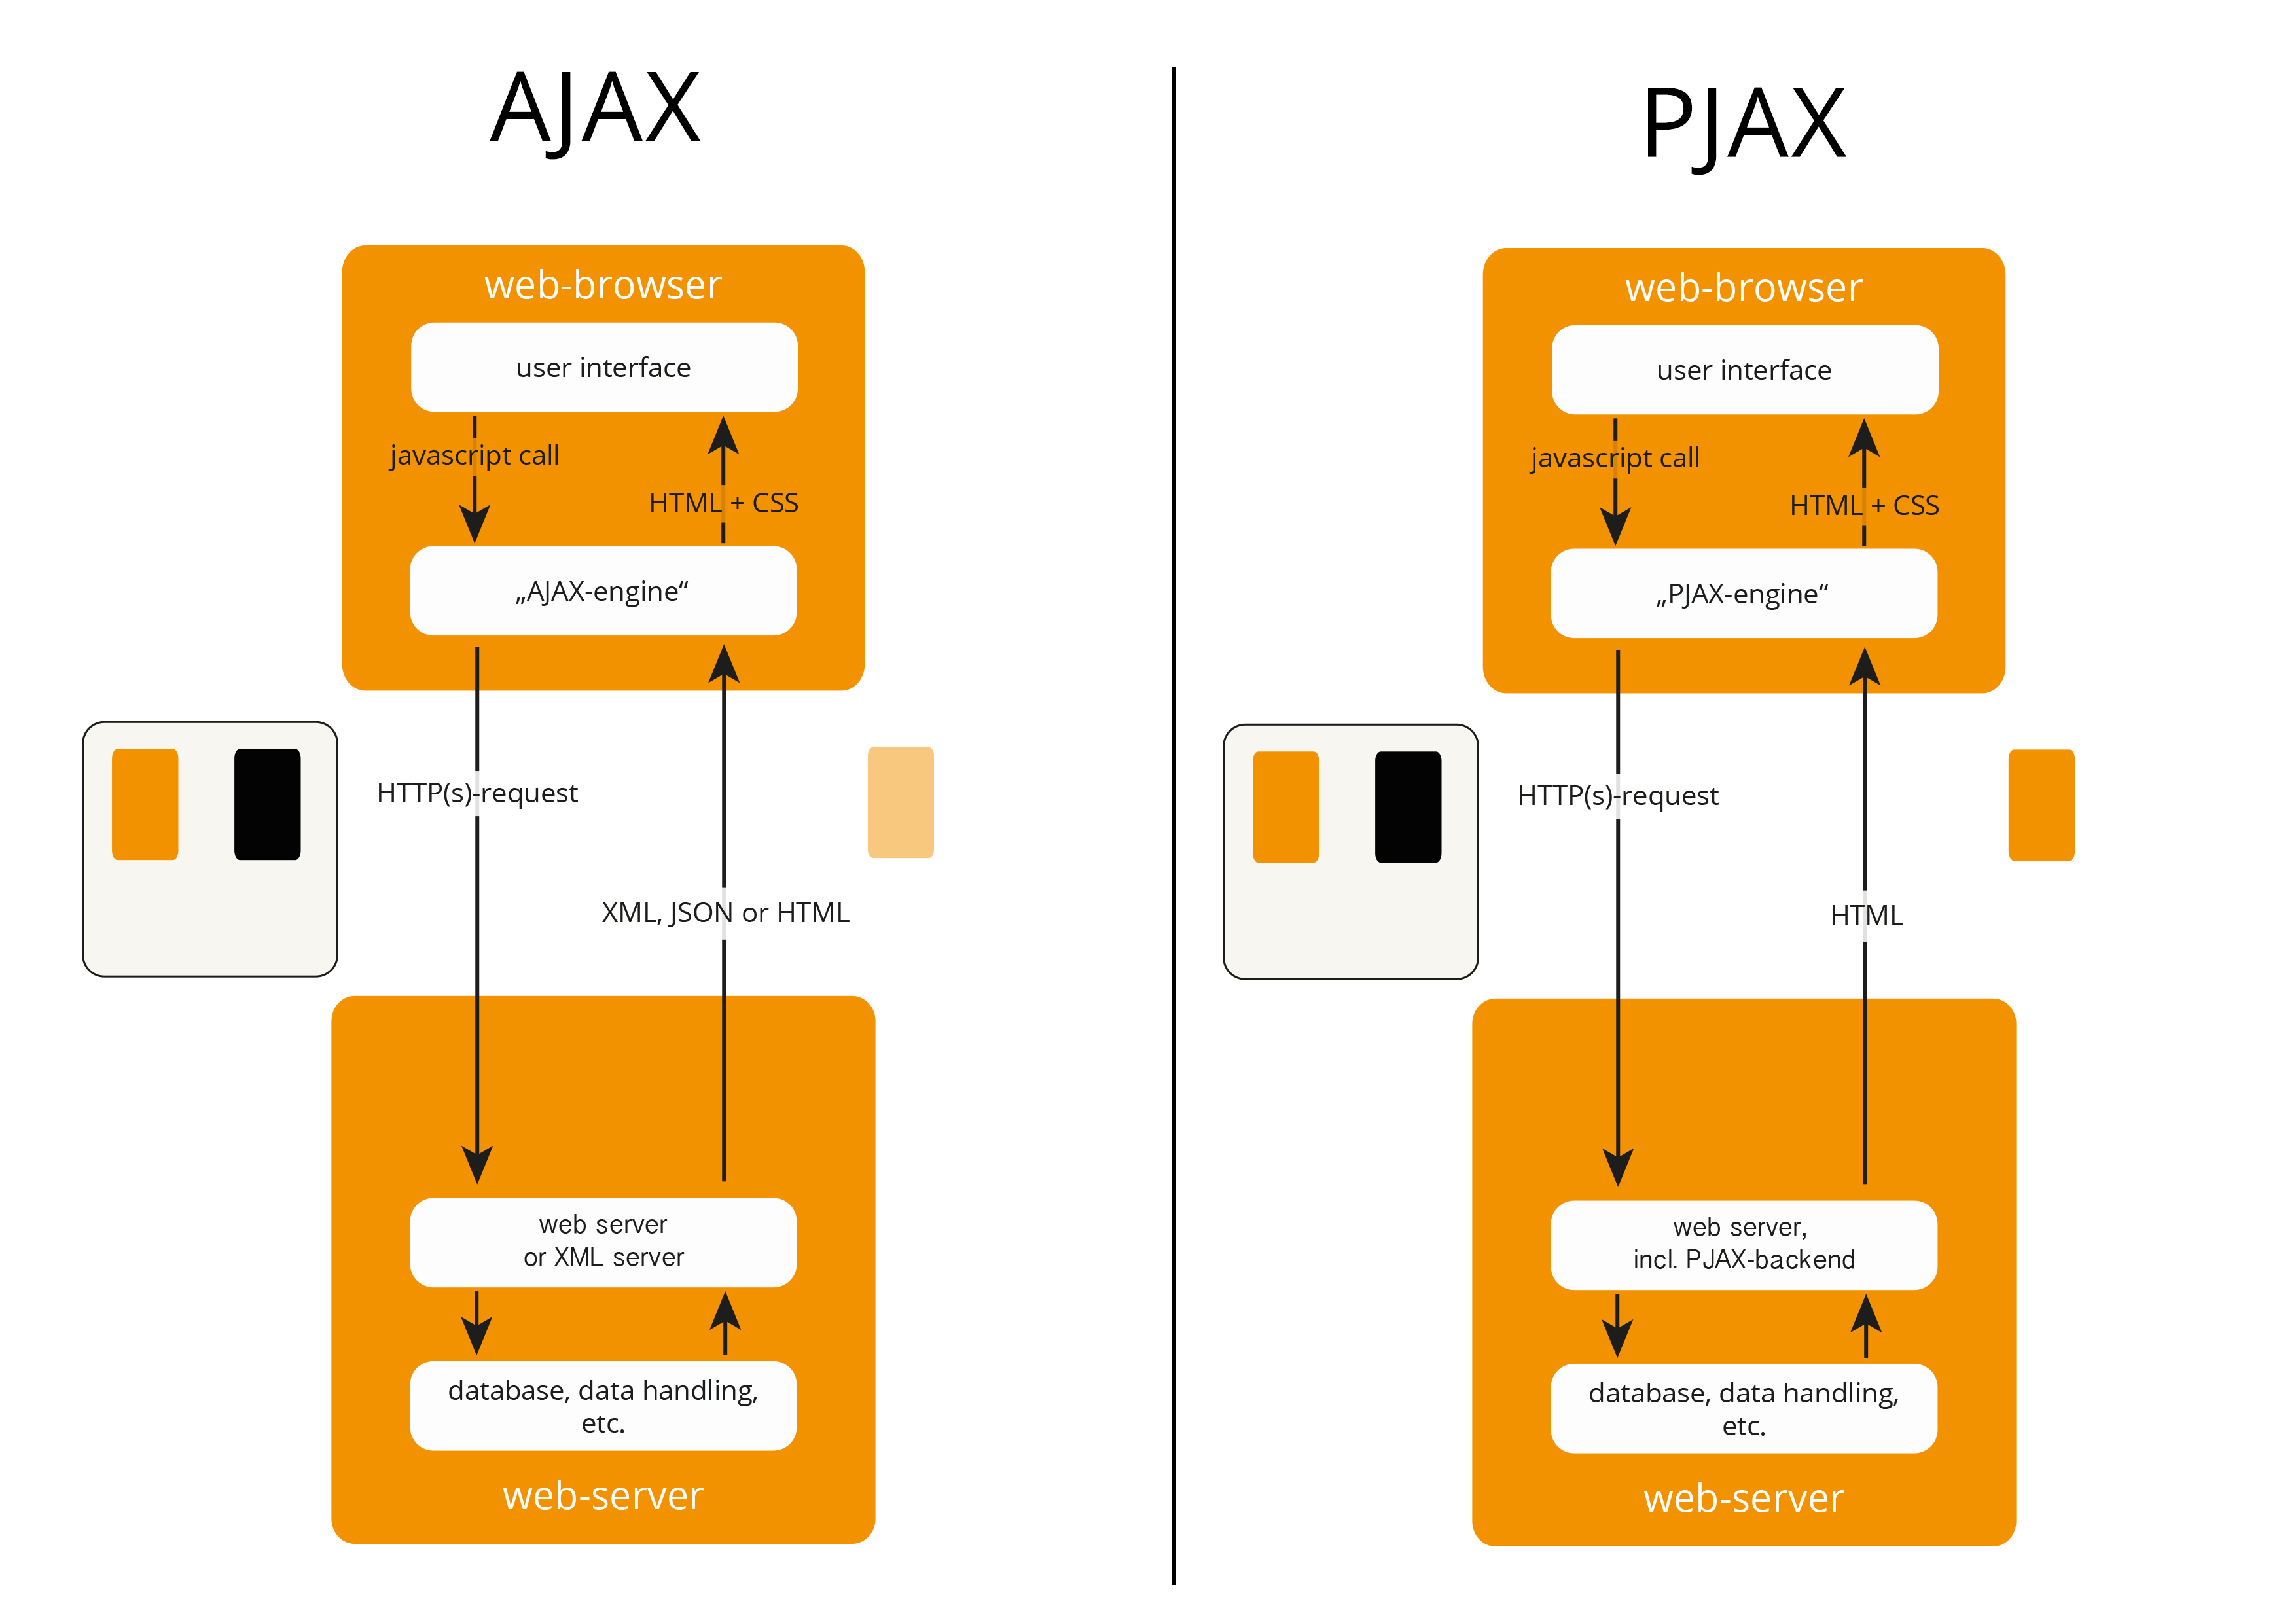
\includegraphics[width=13cm]{images/ajax_vs_pjax}\\
	\enquote{Pushstate Asynchronous JavaScript and XML} is a technique to implement asynchronous requests in a generic way, while still having full browser support.
    Recognizing the problems of \ajax{} the new methods .pushState() and .replaceState() were implemented into modern browsers.
    As described in \ref{theHistoryObject} it allows the website-developer to avoid the disadvantages of \ajax{}:\\
    It's now possible to save the current state of a website and let the browser treat the next changes via \ajax{} like a fully request.
    This means that the back-and forward functionality of your browser is usable again and the current url of your browser changes without having to request a whole new page.\\\\
    The flow of \pjax{} is now:\\
    First an initial request to a web-server is needed using \pjax{}, which is just like the Client-server model, described in \ref{clientServerModel}.
    The changes affect the following requests: 
    The user requests a resource, but now sending an additional HTTP-header which tells the sever it is a \pjaxRequest{}.
    The server interprets and delivers only the needed data in HTML.
    Requesting the same resource without \pjax{} returns you the whole page, containing the content of a \pjaxRequest{} plus everything which is the content which is left out in a \pjaxRequest{}.
    Note that \pjax{} and \pjaxr{} is meant to be integrated as a method to change pages more efficiently.
    For page-independent content, which is not linked to a URL, like a like-button or live-updated stocks pure \ajax{} is still needed.

    \subsubsection{Load time analysis}
      In a case of only one small part of the page needs to be updated, \pjax{} is as efficient as \ajax{}, which means it is about 50ms per request.
      But if you have a complex web-platform you need to update nearly the complete page which leads to load times about the same like the Client-server-model, except the scripts and images which will not invalidate via \pjax{}.
    
    \subsubsection{Requirements}
    \pjax{} needs an additional switch in the HTTP-Server.
    The backend has to decide whether the incoming request is a \pjaxRequest{} or not and then render the data into either the normal template, or the \pjax{}-template.
    On client side only the jquery-pjax library has to be included and activated and the interpretation of the responses are handled by it.

    \subsubsection{Example}
    TODO

    \subsubsection{Pro / Contra}
      \begin{itemize}
  	    \item[+]{The browser functionality is supported completely, especially the back- and forward-buttons.}
  	    \item[+]{It's not necessary to implement every \ajax{}-request in the backend and frontend by hand, a generic solution is easily possible.}
  	    \item[+]{A requested page is always reachable under the same URL, no matter if the page was fully loaded or by a \pjaxRequest{}.}
  	    \item[+]{Only one point to maintain templates in the backend, because no frontend template-engine is needed.}
  	    \item[-]{Only one container and so only one individual feature of the website is affected by a \pjaxRequest{}.}
  	    \item[-]{There are a lot of cases in which \pjax{} is not compatible with the website structure, or would not be as efficient as it could.}
      \end{itemize}


  \subsection{\pjaxr{}, \label{pjaxr}}
    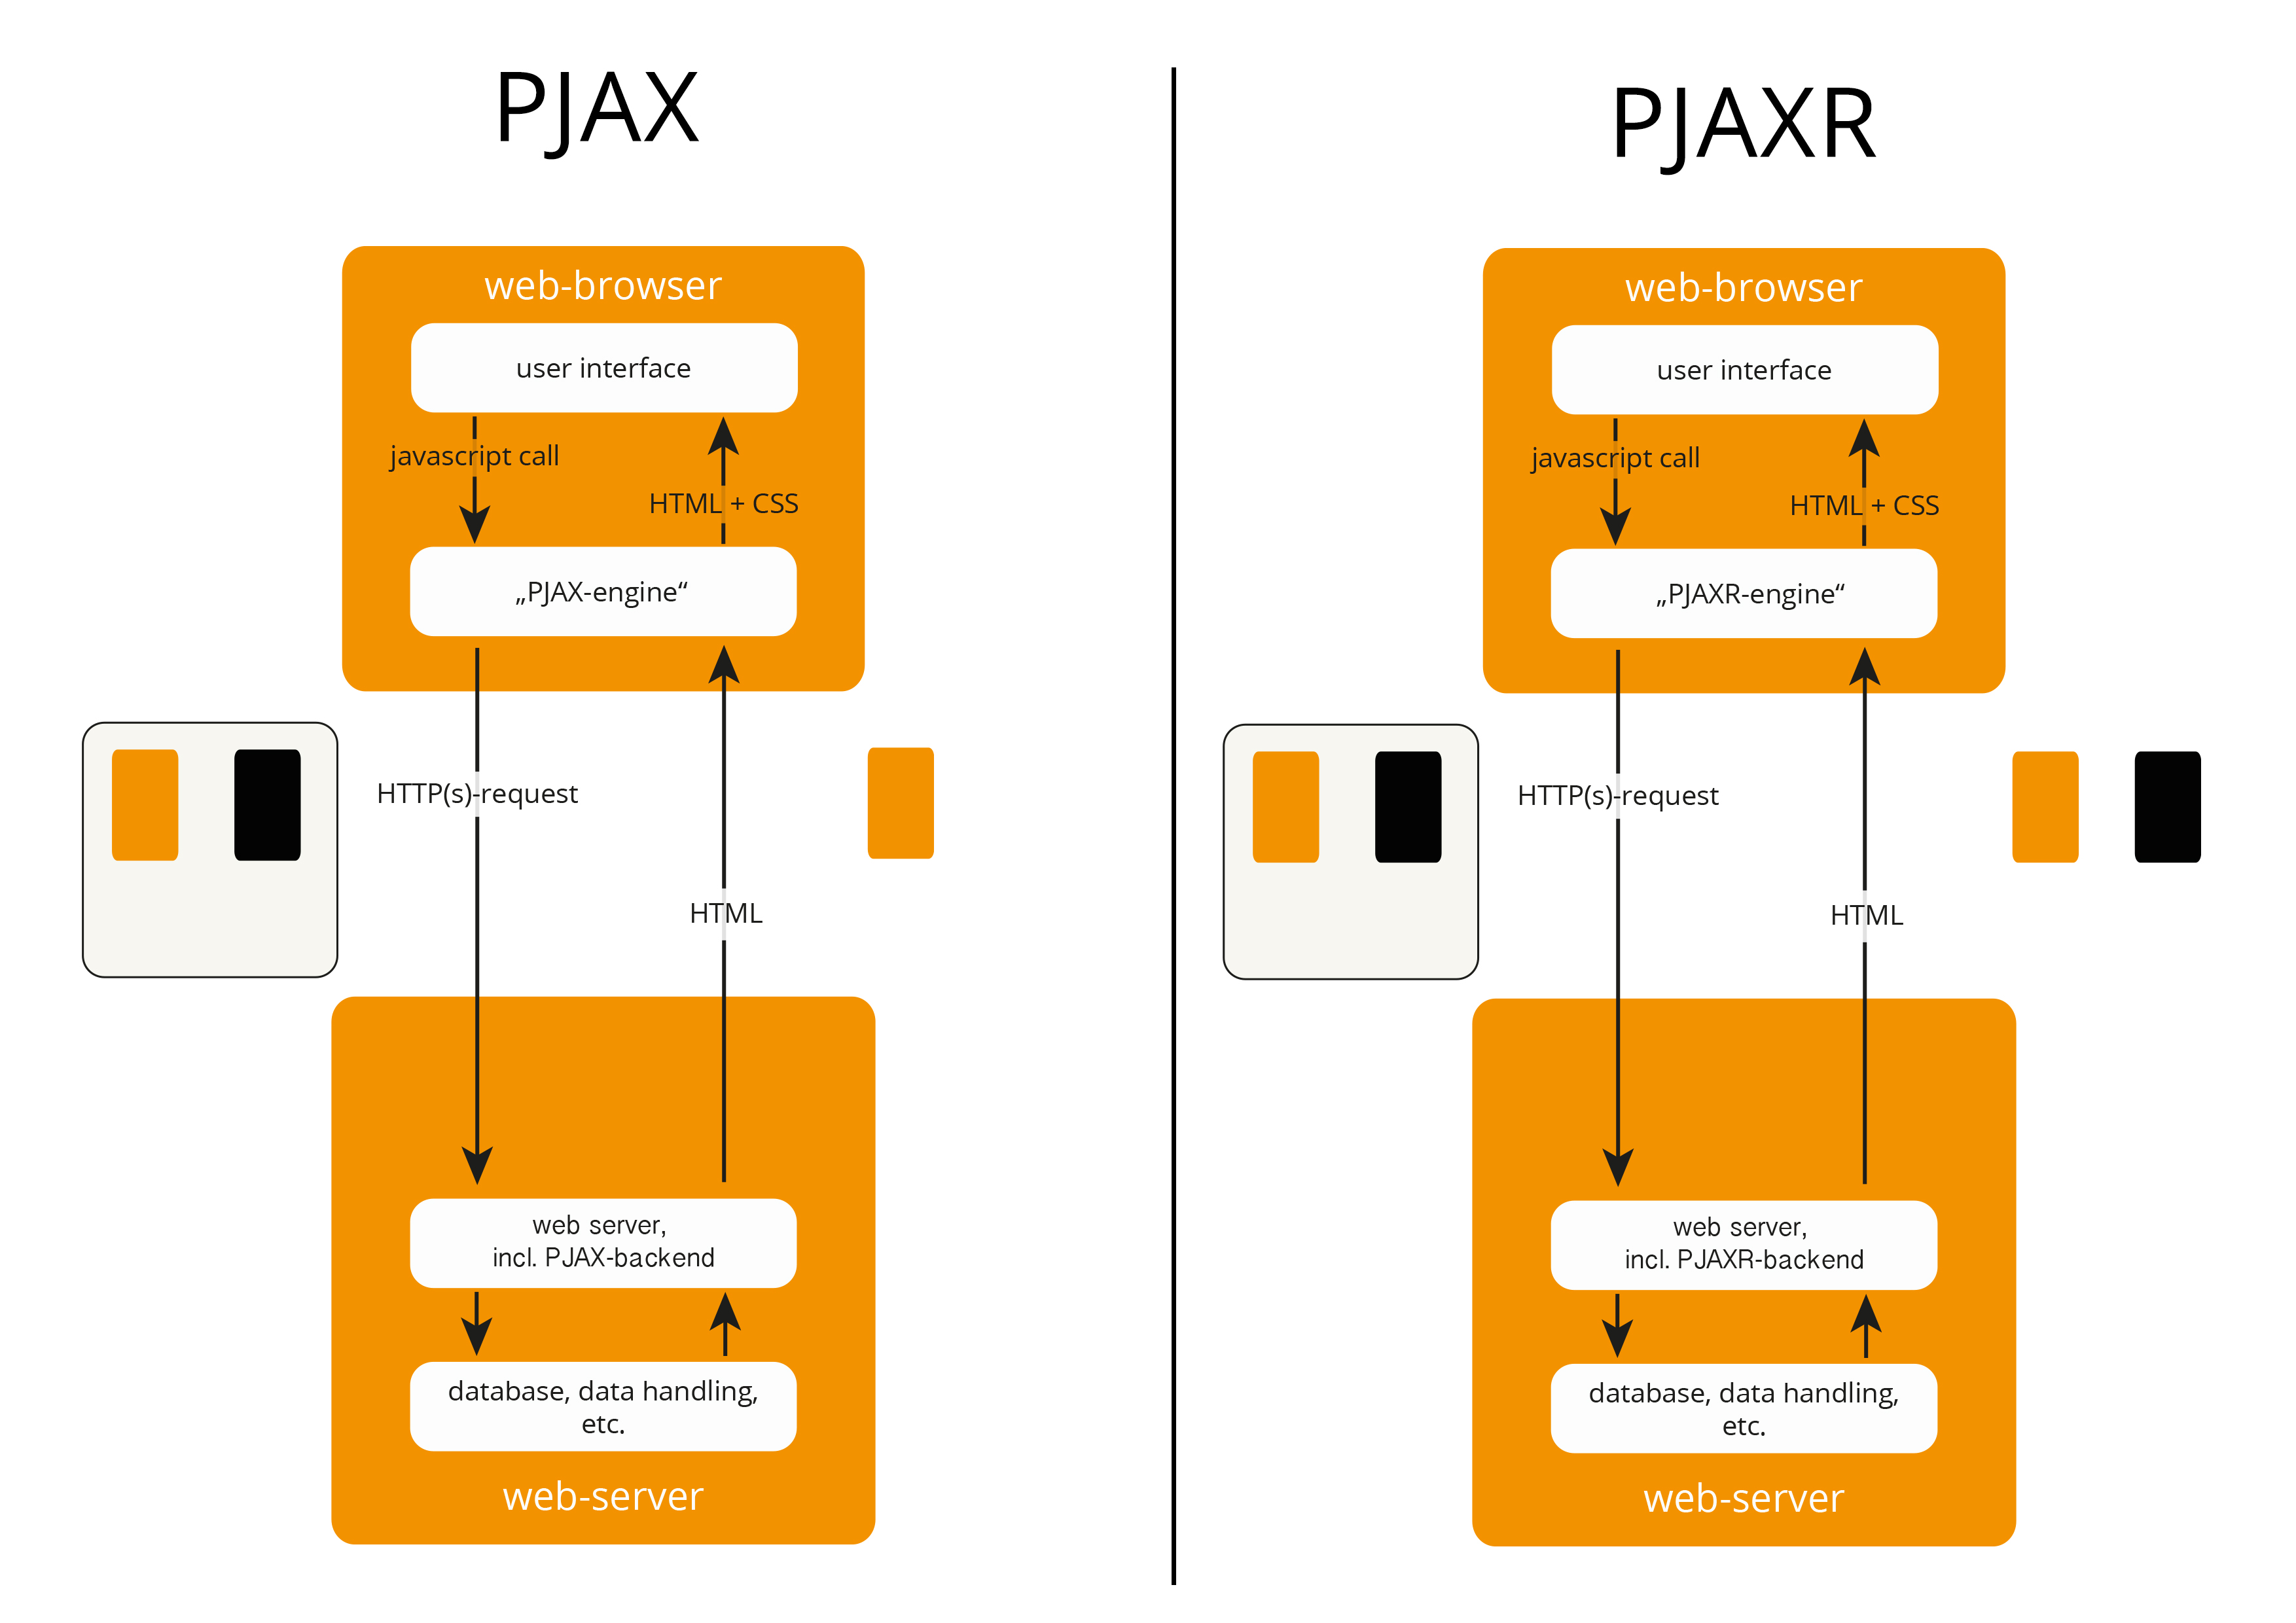
\includegraphics[width=13cm]{images/pjax_vs_pjaxr}\\
    \enquote{Pushstate aJAx eXtended Replacements} is a web-request model which solves \pjax{}'s biggest problem giving the ability of multiple replacements with only one request. 
    Every website has a namespace.
    Sending the current website's namespace as a HTTP-header the \pjaxr{}-backend can decide on which level the current requested website's namespace is matching the one handed through the header.
    According to the match, the server decides in which template the resource should be rendered and requests only the necessary data to render it.
    Other than \pjax{} it does not render and in the frontend replace a specific container, specified before the request, but interprets the response and replaces the received containers with their existing ones.
    As in \pjax{} only one point is necessary to be maintained because you do not have frontend-templating logic.

    \subsubsection{Load time analysis}
      Like \pjax{} the first request takes the same amount of time as every other model.
      But with \pjax{} it's possible to load changing content asynchronously and efficiently with only one request.
      This concludes in a load time of network delay + needed server backends which results in about 75ms for a normal page.
    
    \subsubsection{Requirements}
    \pjaxr{} needs a hierarchical template structure, a \pjaxr{}-backend and on client-side the jquery-pjaxr library has to be included and activated, as in \pjaxr{} the interpretation of the response is made by that library.

    \subsubsection{Example}
    TODO
      
    \subsubsection{Pro / Contra}
      \begin{itemize}
  	    \item[+]{The browser functionality is supported completely, especially the back- and forward-buttons.}
  	    \item[+]{It's not necessary to implement every \ajax{}-request in the backend or  frontend by hand, a generic solution is possible.}
  	    \item[+]{You can replace every container you need in only one \pjaxrRequest{}}
  	    \item[+]{\pjaxr{} can be used on every web-platform using a hierarchical-built template-system.}
  	    \item[+]{Only one point to maintain templates in the backend, because no client-side template-engine is needed.}
        \item[-]{It is not affordable to use \pjaxr{} on finalized projects without a hierarchical template structure, which is necessary.}
      \end{itemize}


  \subsection{Interim conclusion}
  On websites only providing static content the classic Client-server model is as efficient as every other model described above, but it's not possible to have dynamic content on it.
  Pure \ajax{} takes a lot of work to be integrated into larger systems, especially adjusting the client-side interpreter for every resource.
  The more complex a website is, the more the other models take advantage.
  If only one container needs to be changed at a new page, then \pjax{} is a good choice.
  On most sites it's not always the same container to be replaced, on which \pjaxr{} takes it's advantage.\\
  For extremely asynchronous items, for example like-buttons or live-updated content like stocks, which are page-independent features and not linked to a URL pure \ajax{} should be the right choice.

\section{\pjaxr{}}
  TODO
  
  \subsection{Use cases}
  TODO
  
\section{Server-side implementations}
TODO

  \subsection{Java (Spring + Freemarker example)}
  TODO

    \subsection{PHP}
    TODO

\section{Evaluation}
TODO
  
\section{Summary}
TODO

\end{document}
